
\documentclass[a4paper,12pt]{article}
\usepackage{times}
\usepackage[francais]{babel}
\usepackage[utf8x]{inputenc}
\usepackage[T1]{fontenc}
\usepackage{amsmath}
\usepackage{amssymb}
\usepackage{graphicx}
\usepackage{pdfpages}
\usepackage{pdflscape}
\usepackage{listings}
\usepackage{longtable}
\lstset{literate=
{é}{{\'e}}1
{è}{{\`e}}1
{ê}{{\^e}}1
{à}{{\`a}}1
{â}{{\^a}}1
}
\lstset{language=C++,
basicstyle=\footnotesize,
keywordstyle=\footnotesize\color{blue},
otherkeywords={override,nullptr}
}
\definecolor{orange}{rgb}{0.8,0.4,0.0}
\definecolor{darkblue}{rgb}{0.0,0.0,0.6}
\definecolor{cyan}{rgb}{0.0,0.6,0.6}
\lstdefinelanguage{JSON}
{
basicstyle=\normalsize,
columns=fullflexible,
showstringspaces=false,
commentstyle=\color{gray}\upshape,
morestring=[b]",
morestring=[s]{>}{<},
morecomment=[s]{<?}{?>},
stringstyle=\color{orange},
identifierstyle=\color{darkblue},
keywordstyle=\color{blue},
morekeywords={string,number,array,object}% list your attributes here
}

\sloppy

\setlength{\topmargin}{0cm}
\setlength{\headsep}{0.in}
\setlength{\headheight}{0.in}
\setlength{\evensidemargin}{0cm}
\setlength{\oddsidemargin}{-1cm}
\textwidth 18cm
\textheight 25cm

\begin{document}

    \thispagestyle{empty}

    \begin{titlepage}

        \vspace*{2cm}

        \begin{center}\textbf{\Huge Projet Logiciel Transversal}\end{center}{\Large \par}

        \begin{center}\textbf{\large Anand Candassamy \& Paul Estano}\end{center}{\large \par}

        \vspace{2cm}

        \clearpage

        {\small
        \tableofcontents
        }

    \end{titlepage}

    \clearpage
    \section{Présentation Générale}

    \subsection{Archétype}
	    Notre jeu s'inspirera principalement du jeu \emph{Pokemon Donjon Mystère}. En effet, nous avons prévu de conserver le mécanisme des combats et de donjon de ce jeu.
	    \\Dans notre logiciel l'utilisateur incarnera un pokemon dans les salles d'un donjon qui contiennent chacune des pokemons qui peuvent l'"agresser".
	    \\Pour simplifier le jeu nous abandonnons également d'évolution des pokemons.

    \subsection{Règles du jeu}
	  Le donjon contient un nombre fini de salle et le joueur gagne lorsqu'il sort de la dernière salle du donjon.
	   \\Lorsque l'utilisateur est provoqué en duel automatiquement par les pokémons qui sont autour de lui.
\\Les combats fonctionnent en tour par tour. A chaque tour, l'utilisateur peut effectuer qu’une seule action.
\begin{itemize}
    \item attaquer
    \item soigner le pokemon
    \item se déplacer
\end{itemize}
\clearpage
    \subsection{Ressources}
    \begin{figure}[ht]
    \begin{center}
        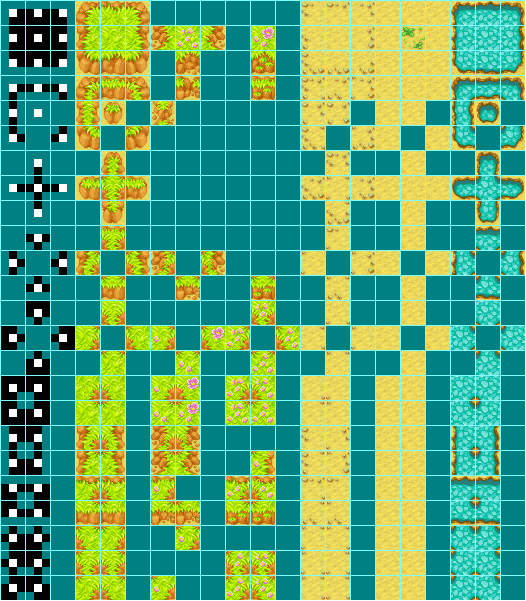
\includegraphics[width=0.8\textwidth]{tilemap.png}
    \end{center}
    \caption{Tileset utilisé pour construire un monde}
    \end{figure}

    \begin{figure}[ht]
    \begin{center}
        
\includegraphics[width=0.8\textwidth]{pokemonLatex.png}
    \end{center}
    \caption{Tileset utilisé pour les pokémons}
    \end{figure}



    \clearpage
    \section{Description et conception des états}

    \subsection{Description des états}
    Un état du jeu est formé d'une carte qui est statique au cours du temps et d'une liste de joueurs dont l'état varie au cours du jeu.

    \subsubsection{Etat de la carte}
    Une carte est composée de : \begin{itemize}
        \item plusieurs couches
        \item d'une longueur en nombre de tiles
        \item d'une largeur en nombre de tiles
        \item de la largeur de ses tiles en pixels
        \item de la longueur de ses tiles en pixels
        \item d'un tileset
    \end{itemize}
    Une tile correspond à un motif de pixels utilisé sur une ou plusieurs cases de la carte par une ou plusieurs couches.

    Chaque couche de la carte comporte:\begin{itemize}
        \item un nom
        \item une largeur en nombre de tiles
        \item une longueur en nombre de tiles
        \item une position correspondant à la position de sa première case
        \item une liste d'index correspondant aux tiles utilisé pour chaque case. Ces tiles doivent se trouver dans le tileset de la carte
    \end{itemize}

    Un tileset comprend :  une chaîne de caractères correspondant au chemin de l'image du tileset et un identifiant.

    \subsubsection{État des joueurs}
    Un joueur est soit vivant, soit mort, soit un robot, soit un humain et il lui est attribué un pokemon en début de partie.

    Un pokemon possède une position, un nombre de points de vie à l'état t, un nom et un ensemble de statistiques qui lui sont attribués en début de partie.

    Ces statistiques correspondent aux attaques qu'il peut utiliser, à son nombre de point de vie en début de partie et son type (eau, feu, herbe).
    \subsection{Conception Logiciel}
    Le package état peut se diviser en trois sous-partie:\begin{itemize}
        \item Une partie gérant les personnages, en bleu
        \item Une partie gérant l'environnement, en rouge
        \item Une classe représentant l'état global du jeu, en vert
    \end{itemize}

    La classe \emph{player} contient l'ensemble des éléments permettant de caractériser l'état d'un joueur. Chaque joueur est lié à un pokemon par une relation de composition : un pokémon ne peut pas exister sans joueur. Dans le cas où le pokémon est contrôlé par l'IA, l'IA est considérée comme un joueur.
    \\Chaque pokémon possède une relation d'agrégation avec des statistiques qui lui sont attribués en début de partie.
    \\La partie environnement est calqué sur le modèle proposé par les fichiers exporter par le logiciel \emph{Tiled Map Editor}. Les objets les plus consommateurs en mémoire tels les \emph{data} dans la classe \emph{Layer} sont par ailleurs stockés dans le tas pour éviter les copies entre les différentes classes.
    \\L'état global contient un pointeur vers l'état de l'environnement et et une liste de pointeur de contenant l'état des différents joueurs de la partie.
    \begin{landscape}
    \begin{figure}[p]
    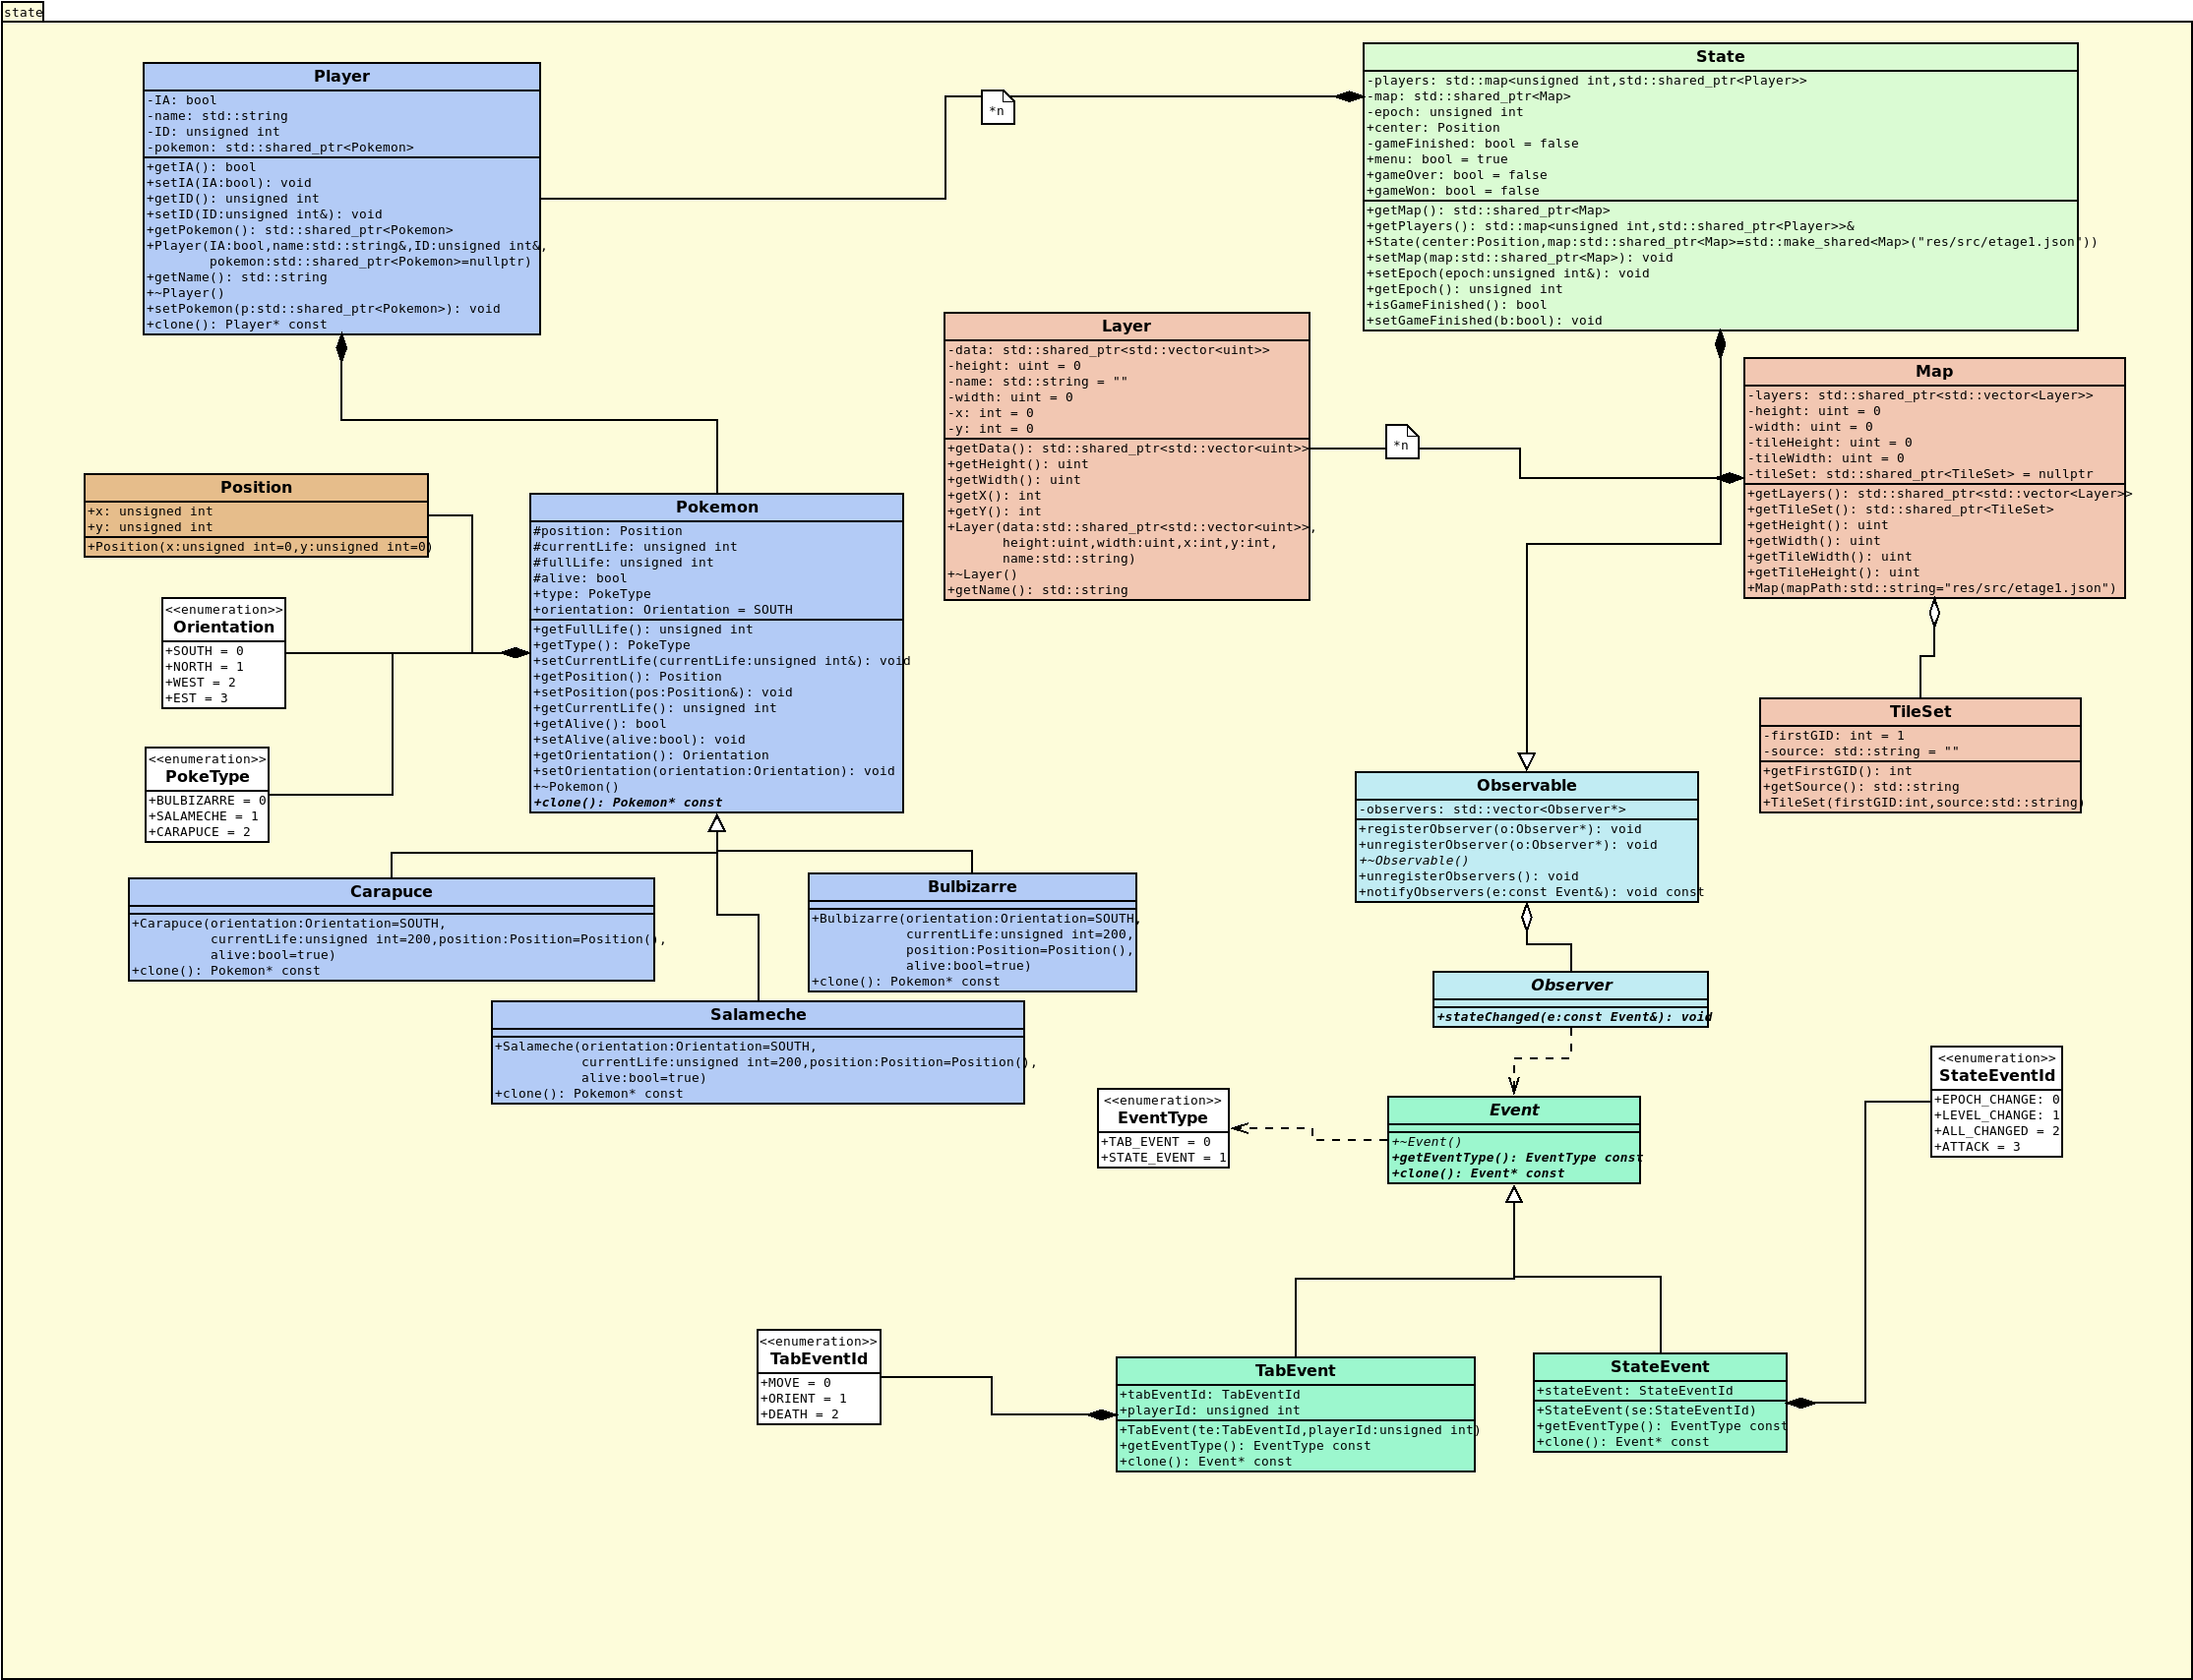
\includegraphics[width=0.8\paperheight]{state.png}
    \caption{\label{uml:state}Diagramme des classes d'état.}
    \end{figure}
    \end{landscape}
    \clearpage


    \section{Rendu: Stratégie et Conception}

    \subsection{Stratégie de rendu d'un état}


    \subsection{Conception logiciel}

    %\begin{landscape}
    %\begin{figure}[p]
    %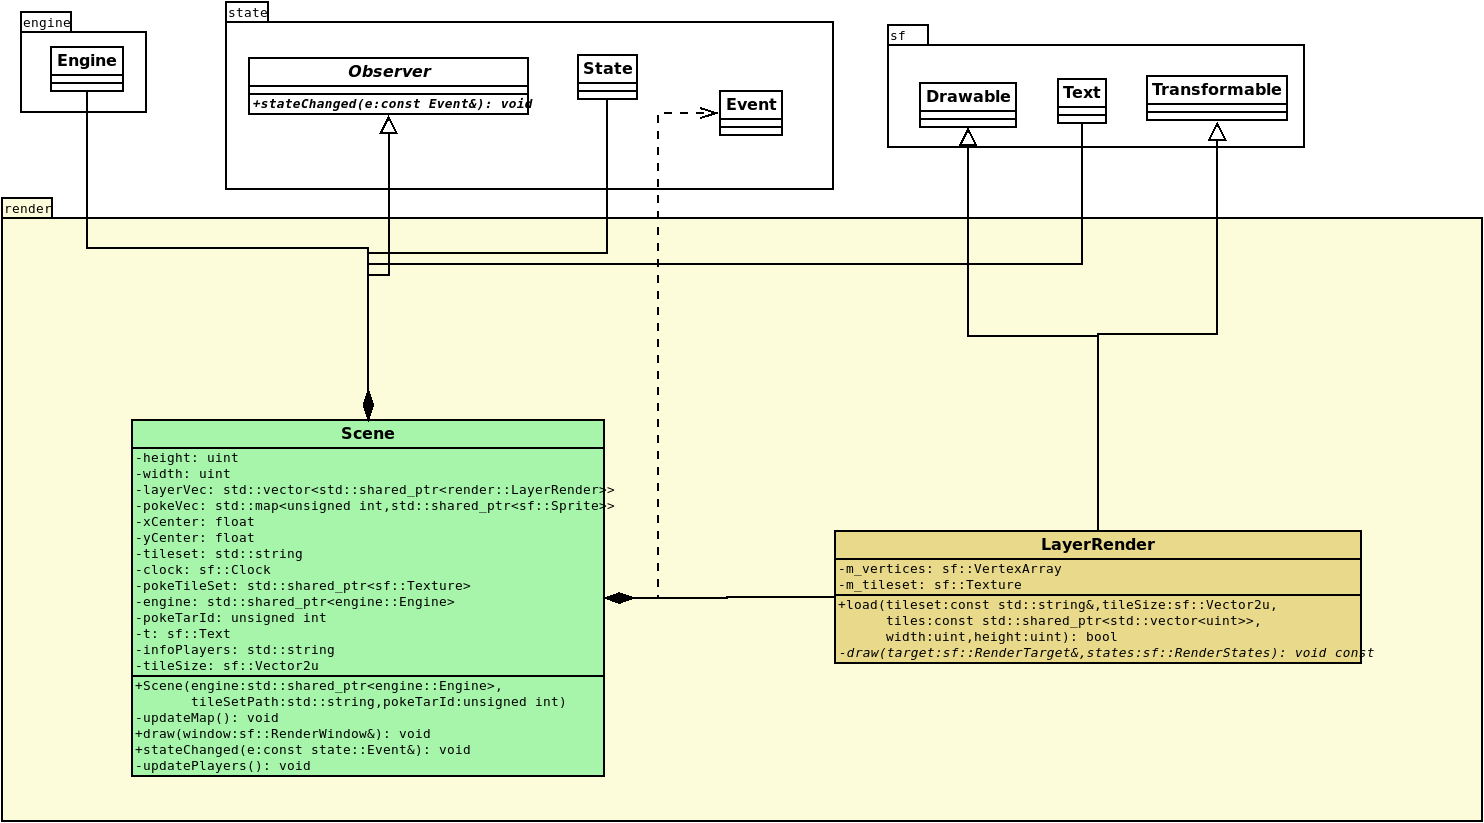
\includegraphics[width=0.9\paperheight]{render.pdf}
    %\caption{\label{uml:render}Diagramme des classes de rendu.}
    %\end{figure}
    %\end{landscape}

    \clearpage
    \section{Règles de changement d'états et moteur de jeu}

    \subsection{Règles}

    \clearpage
    \subsection{Conception logiciel}


    %\begin{landscape}
    %\begin{figure}[p]
    %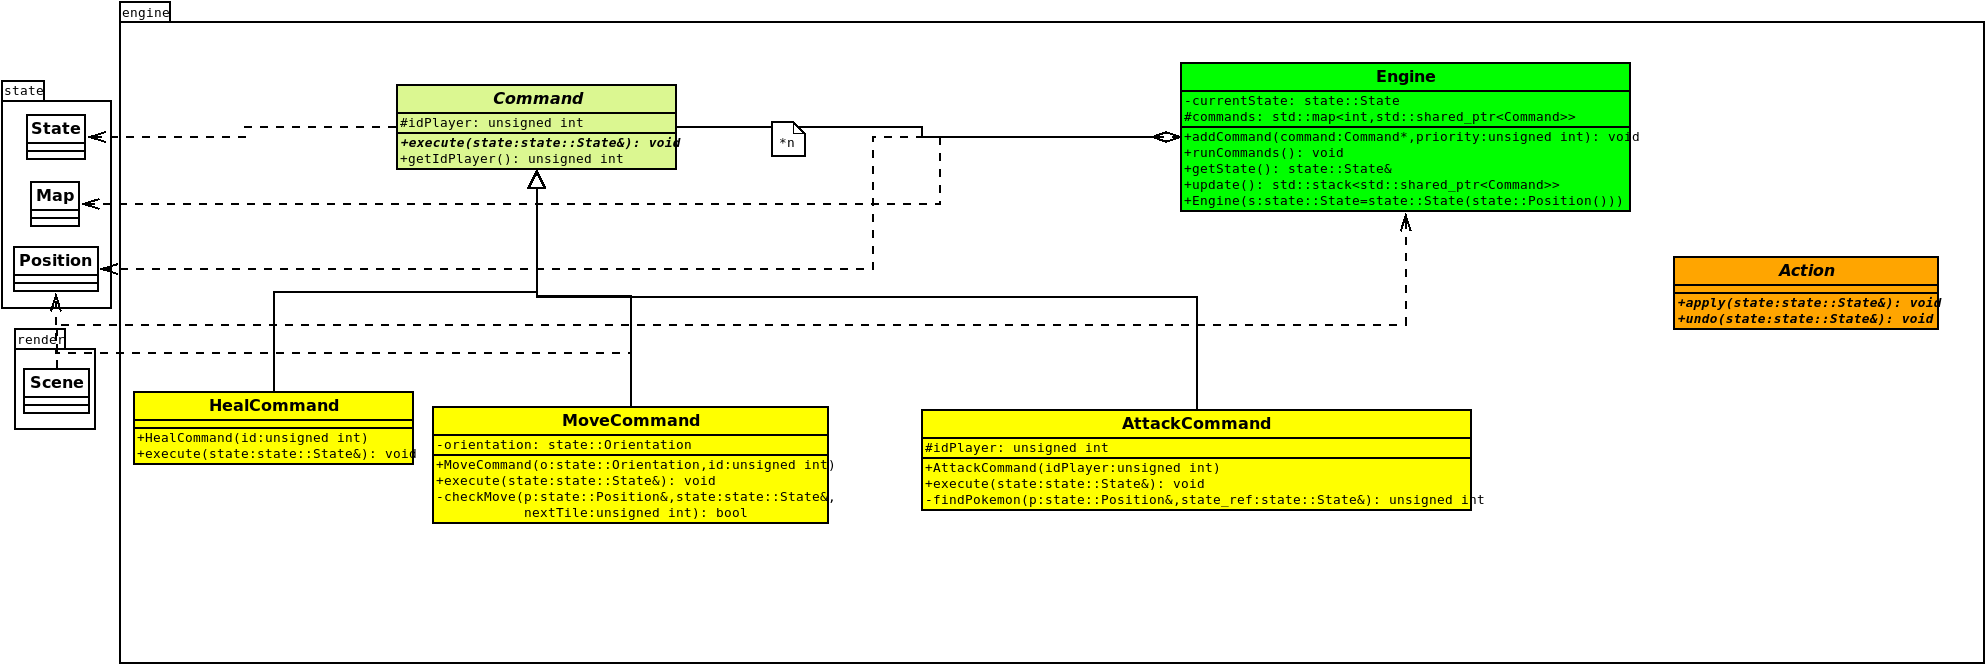
\includegraphics[width=0.9\paperheight]{engine.pdf}
    %\caption{\label{uml:engine}Diagramme des classes de moteur de jeu.}
    %\end{figure}
    %\end{landscape}


    \section{Intelligence Artificielle}

    \subsection{Stratégies}

    \clearpage
    \subsection{Conception logiciel}


    %\begin{landscape}
    %\begin{figure}[p]
    %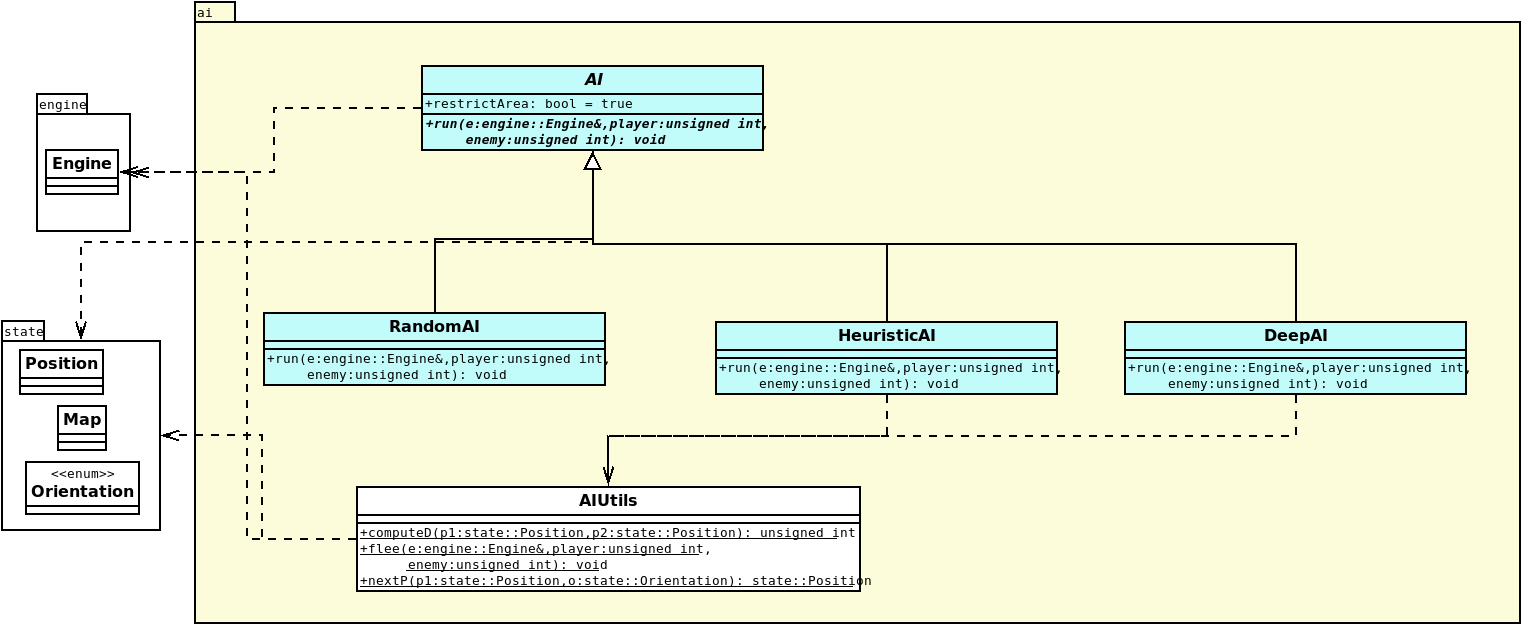
\includegraphics[width=0.9\paperheight]{ai.pdf}
    %\caption{\label{uml:ai}Diagramme des classes d'intelligence artificielle.}
    %\end{figure}
    %\end{landscape}


    \section{Modularisation}
    \label{sec:module}

    \subsection{Organisation des modules}

    \clearpage
    \subsection{Conception logiciel}


    %
    %\begin{landscape}
    %\begin{figure}[p]
    %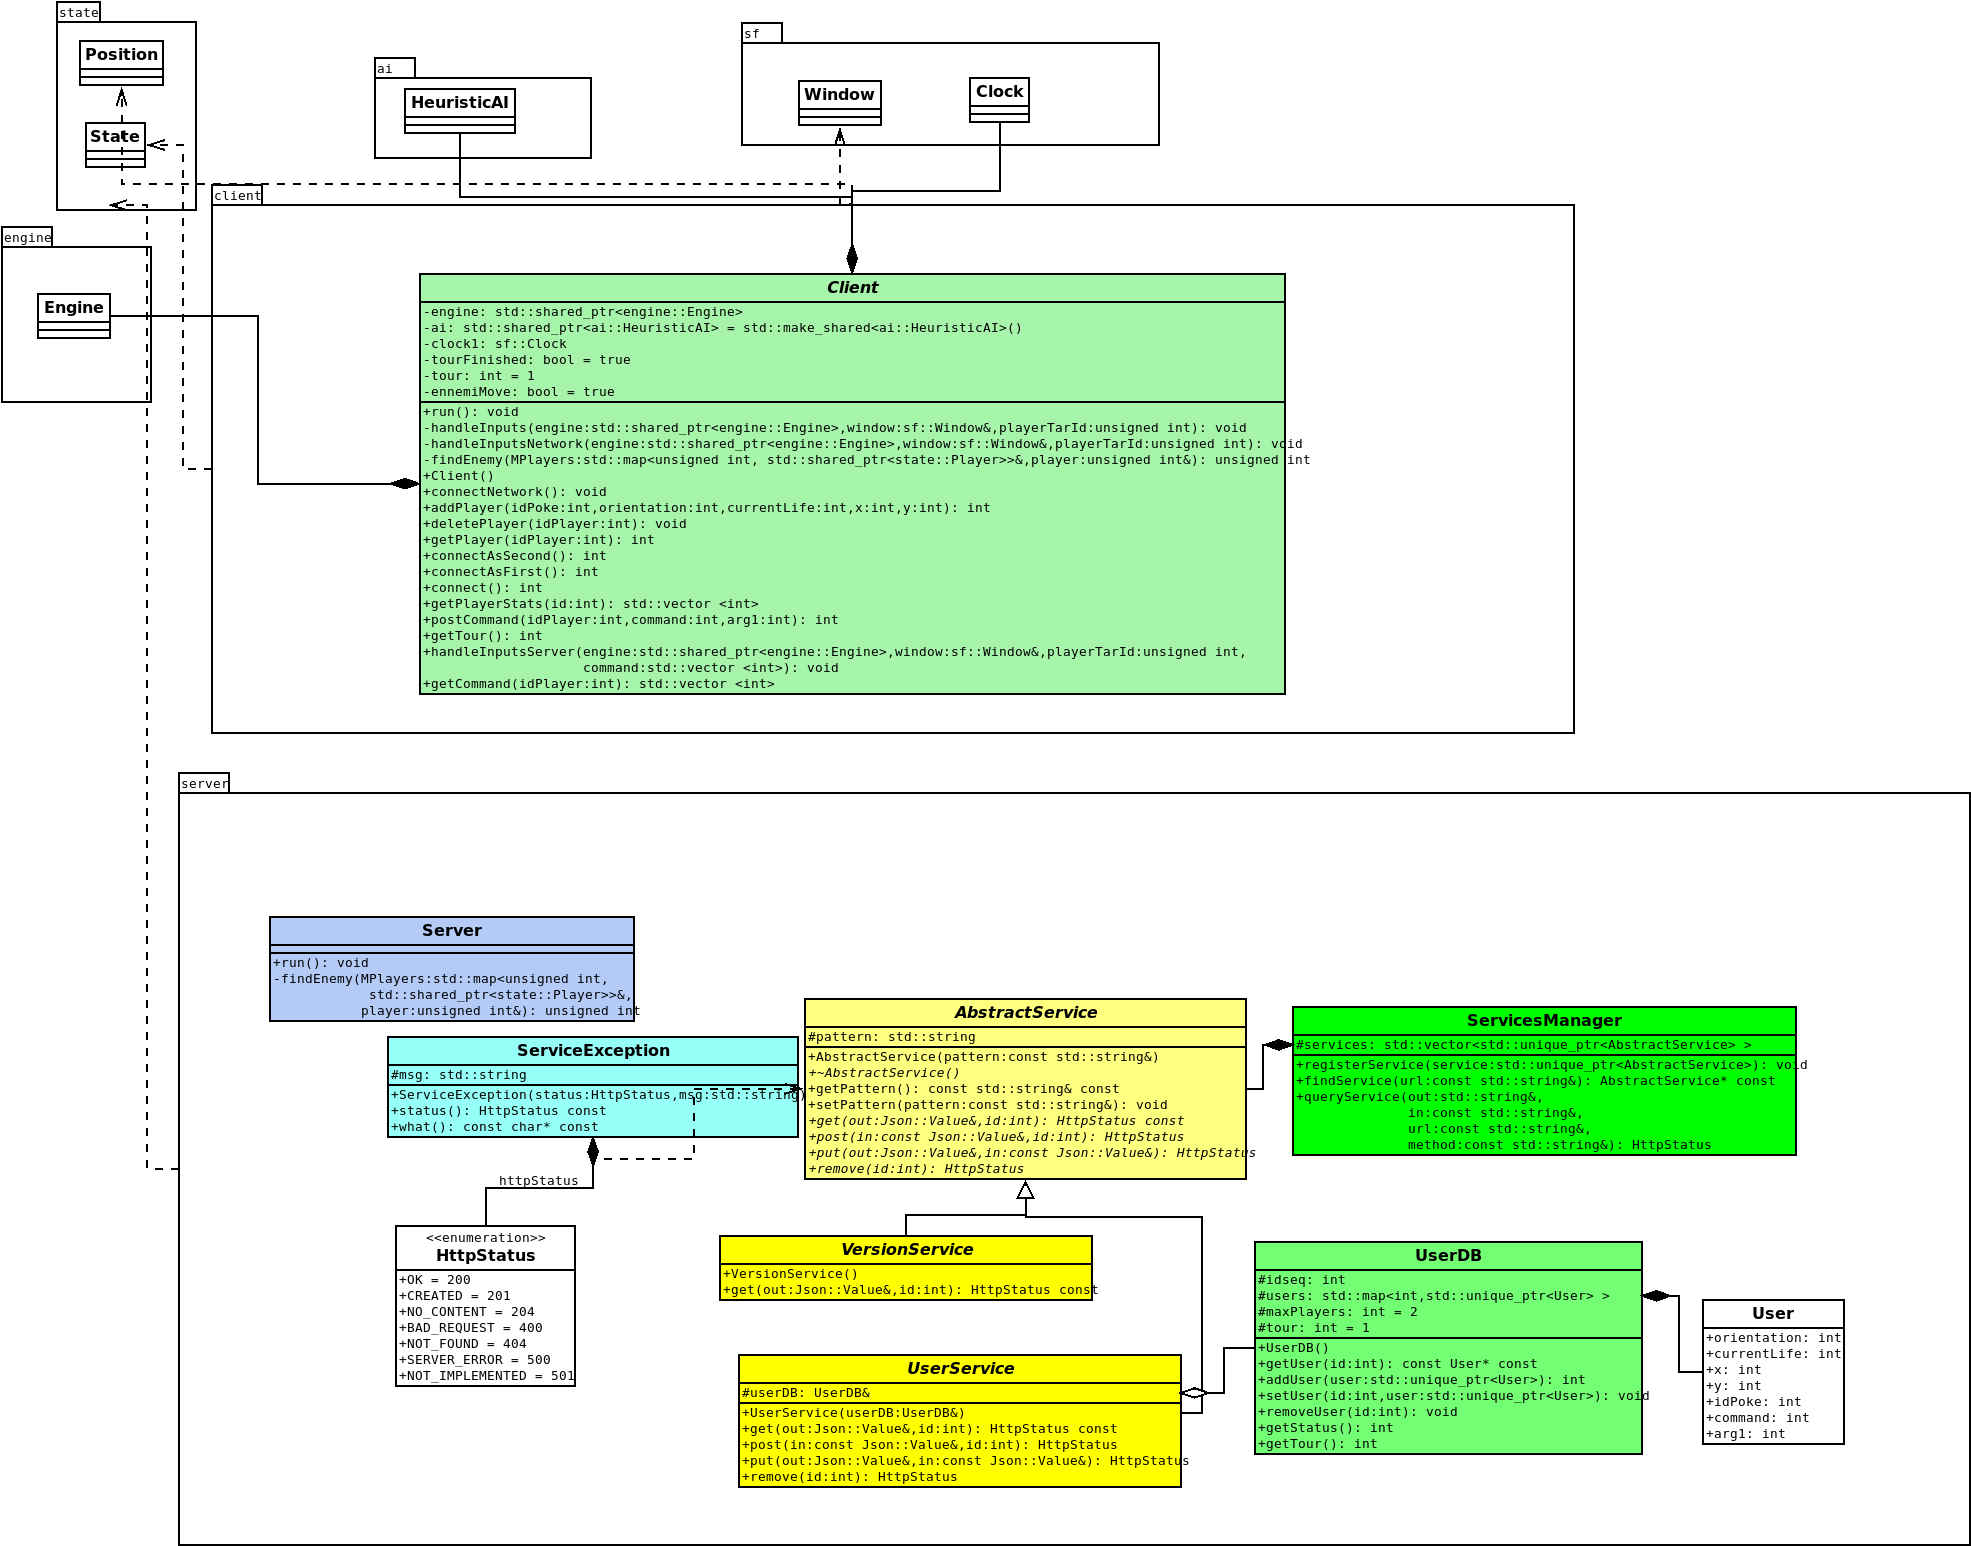
\includegraphics[width=0.9\paperheight]{module.pdf}
    %\caption{\label{uml:module}Diagramme des classes pour la modularisation.}
    %\end{figure}
    %\end{landscape}

\end{document}
